\documentclass[12pt]{article}
\usepackage{geometry}
\geometry{a4paper, total={170mm, 250mm}}
\title{\textbf{Homework 4}}
\author{Maedeh Karkhane Yousefi}
\usepackage{float}
\usepackage{graphicx}
\usepackage{subcaption}
\begin{document}
\maketitle
\part*{1. Exercise 4.5,4.6: Correlation Length }
\paragraph*{} We are supposed to obtain the correlation length in each run for the previous code using the HK algorithm (exercise 4.4). I added the function \textit{RadiusOfGyration}, which finds the maximum finite cluster and according to it's size and the related label, finds all the entries that are in this cluster, gets their indices, and their center of masses respectively. At last, the distance of all the entries from the center of mass is calculated, and the radius of Gyration is obtained accordingly. 
For each length in the list, we run the program for 1000 times, and the mean and STD of the Radius of Gyrations ($\xi$) is calculated.
\paragraph*{} In order to get the amounts $\nu$ and $P_{c}(\infty)$, I used the package \textit{LsqFit} and the \textit{curve$\_$fit} method subsequently. Putting the equation( $\left|p_{c}(L)-P_{c}(\infty)\right|^{-\nu} \sim L$ ) as the \textit{model}. The critical values of probability for each length were resulted from the achieved data, and the preassumed values for $\nu$ and $P_{c}(\infty)$ are 0.59 and 1.3, respectively.
\paragraph*{} results from \textit{curve$\_$fit} are: $\nu \sim 0.61$ , $ P_{c}(\infty) \sim 1.02$
\begin{figure}[H]
	\centering
	\begin{subfigure}[t]{0.8\textwidth}
		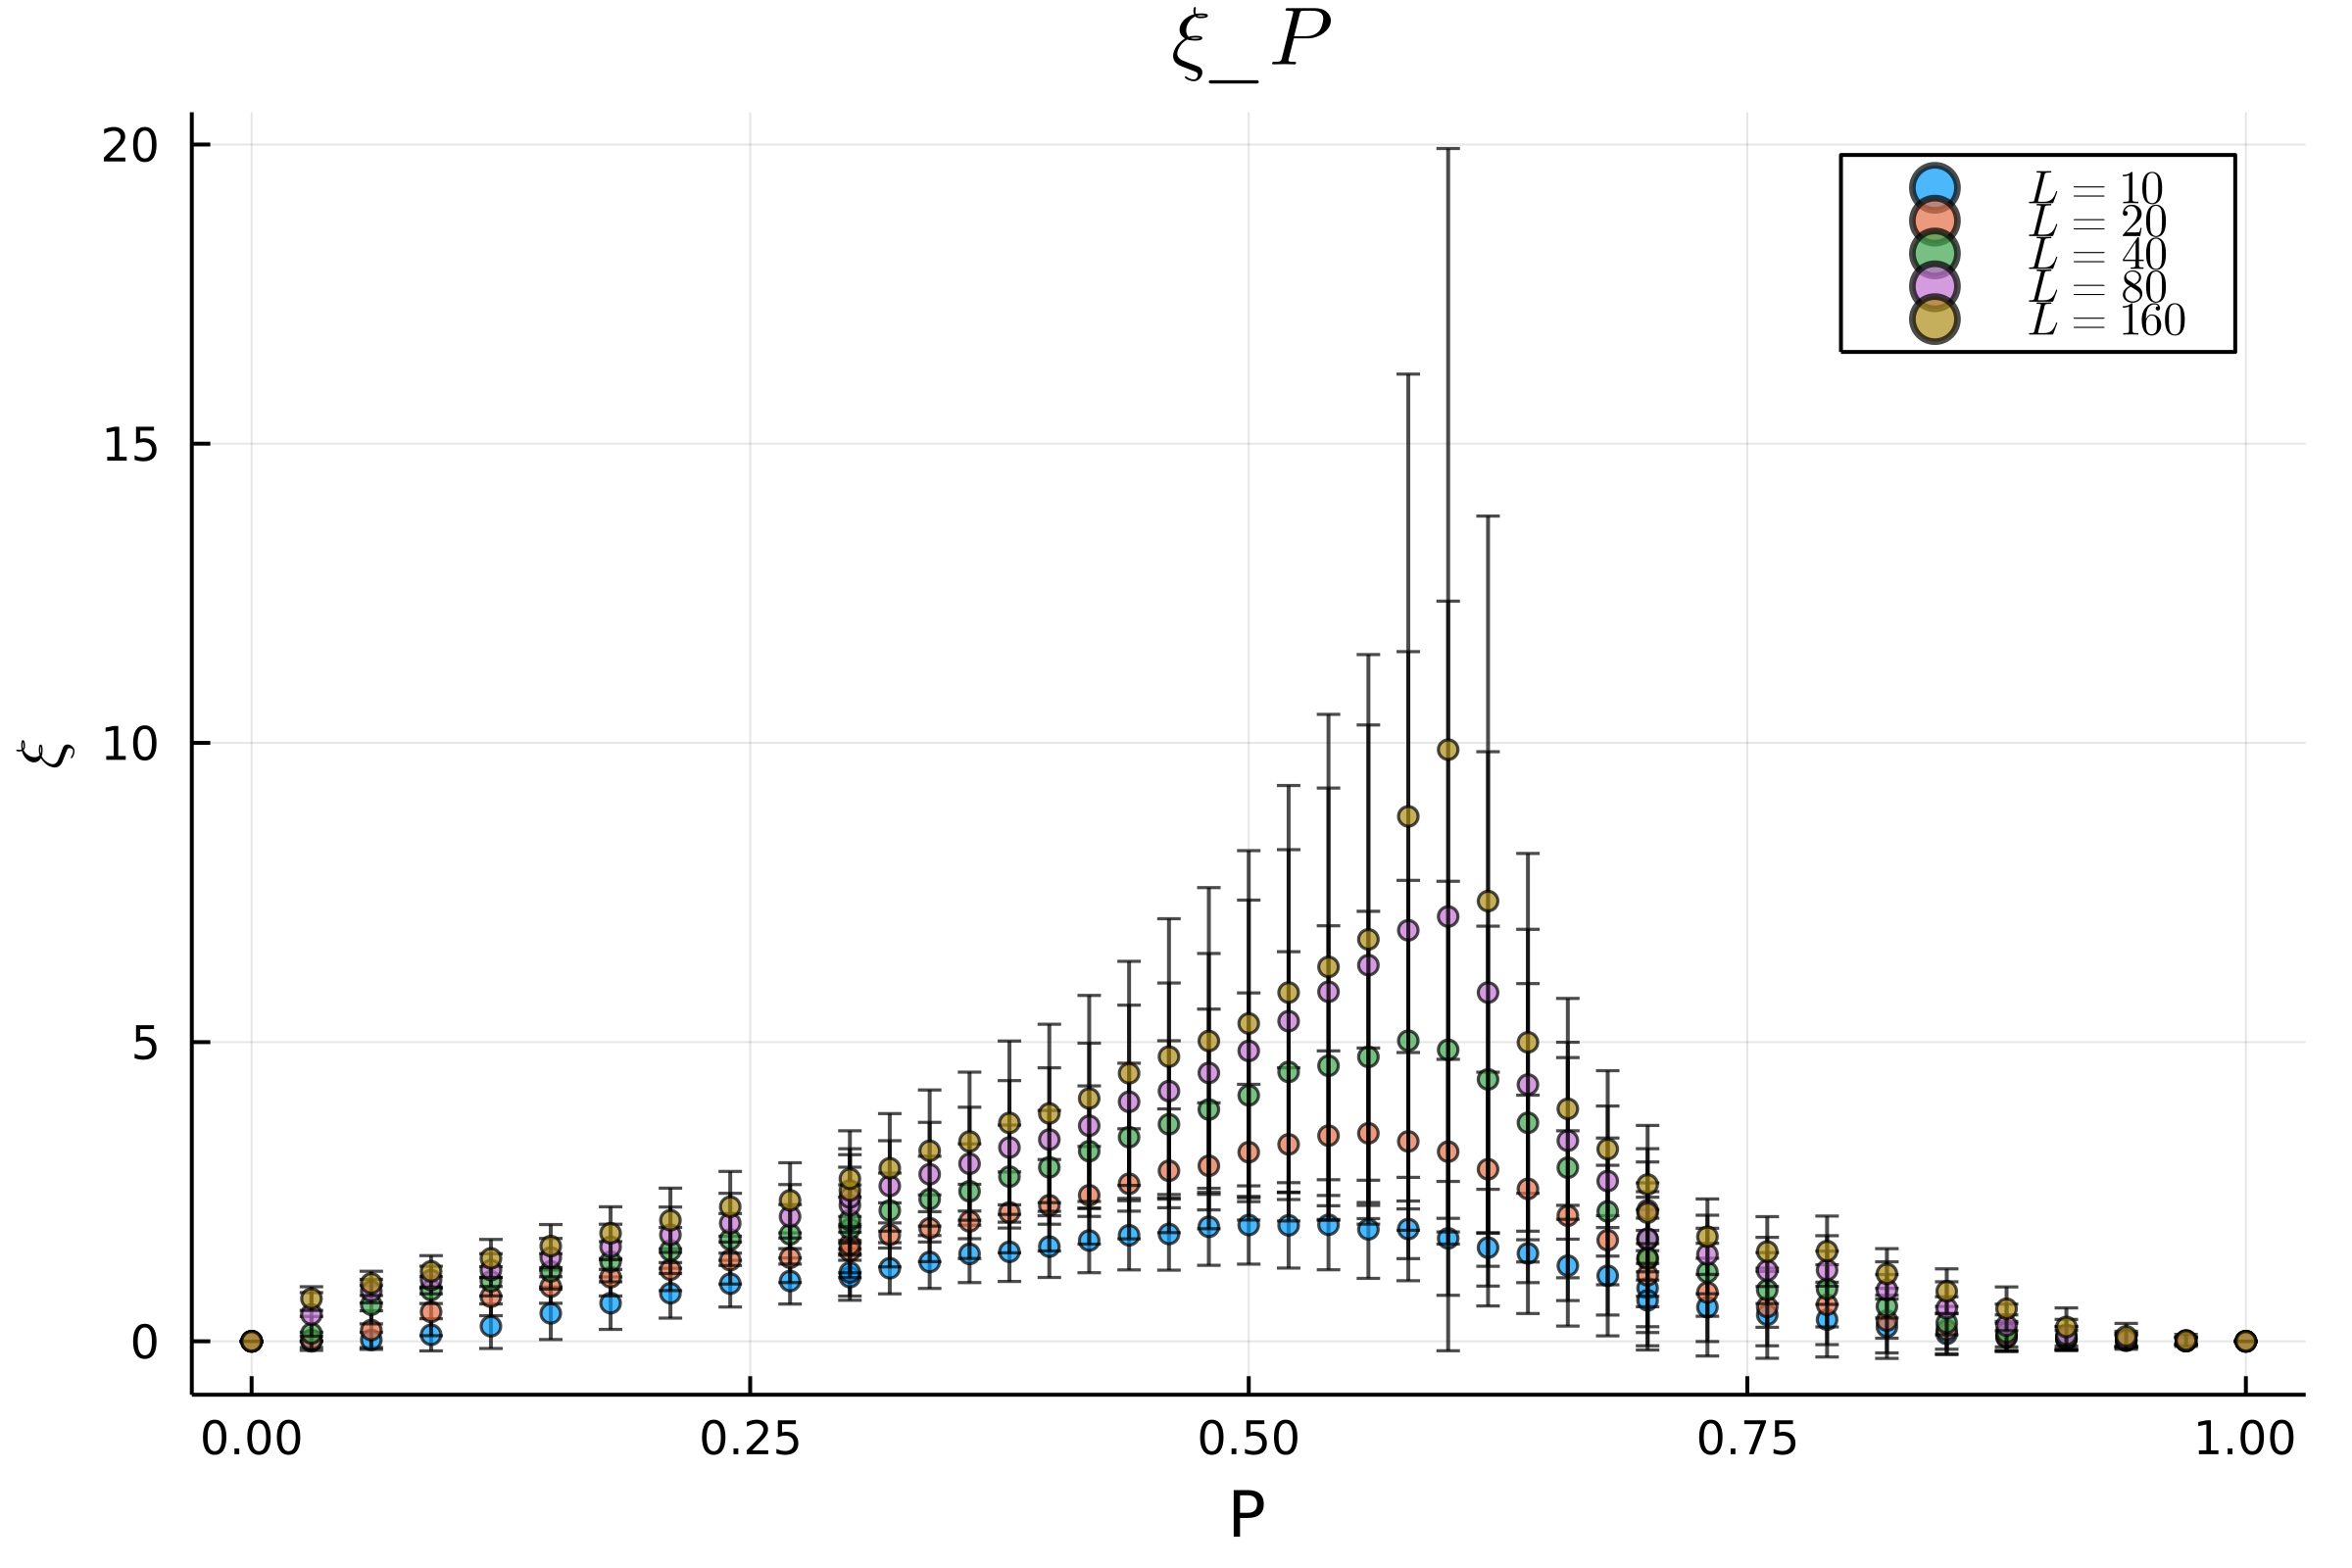
\includegraphics[width=\textwidth]{4.5_scatter.png}
		\label{fig:mesh1.1}
		\caption{The scatter $\xi$ over probability figure (error bars included).}
	\end{subfigure}\par\bigskip 
	\begin{subfigure}[t]{0.8\textwidth}
		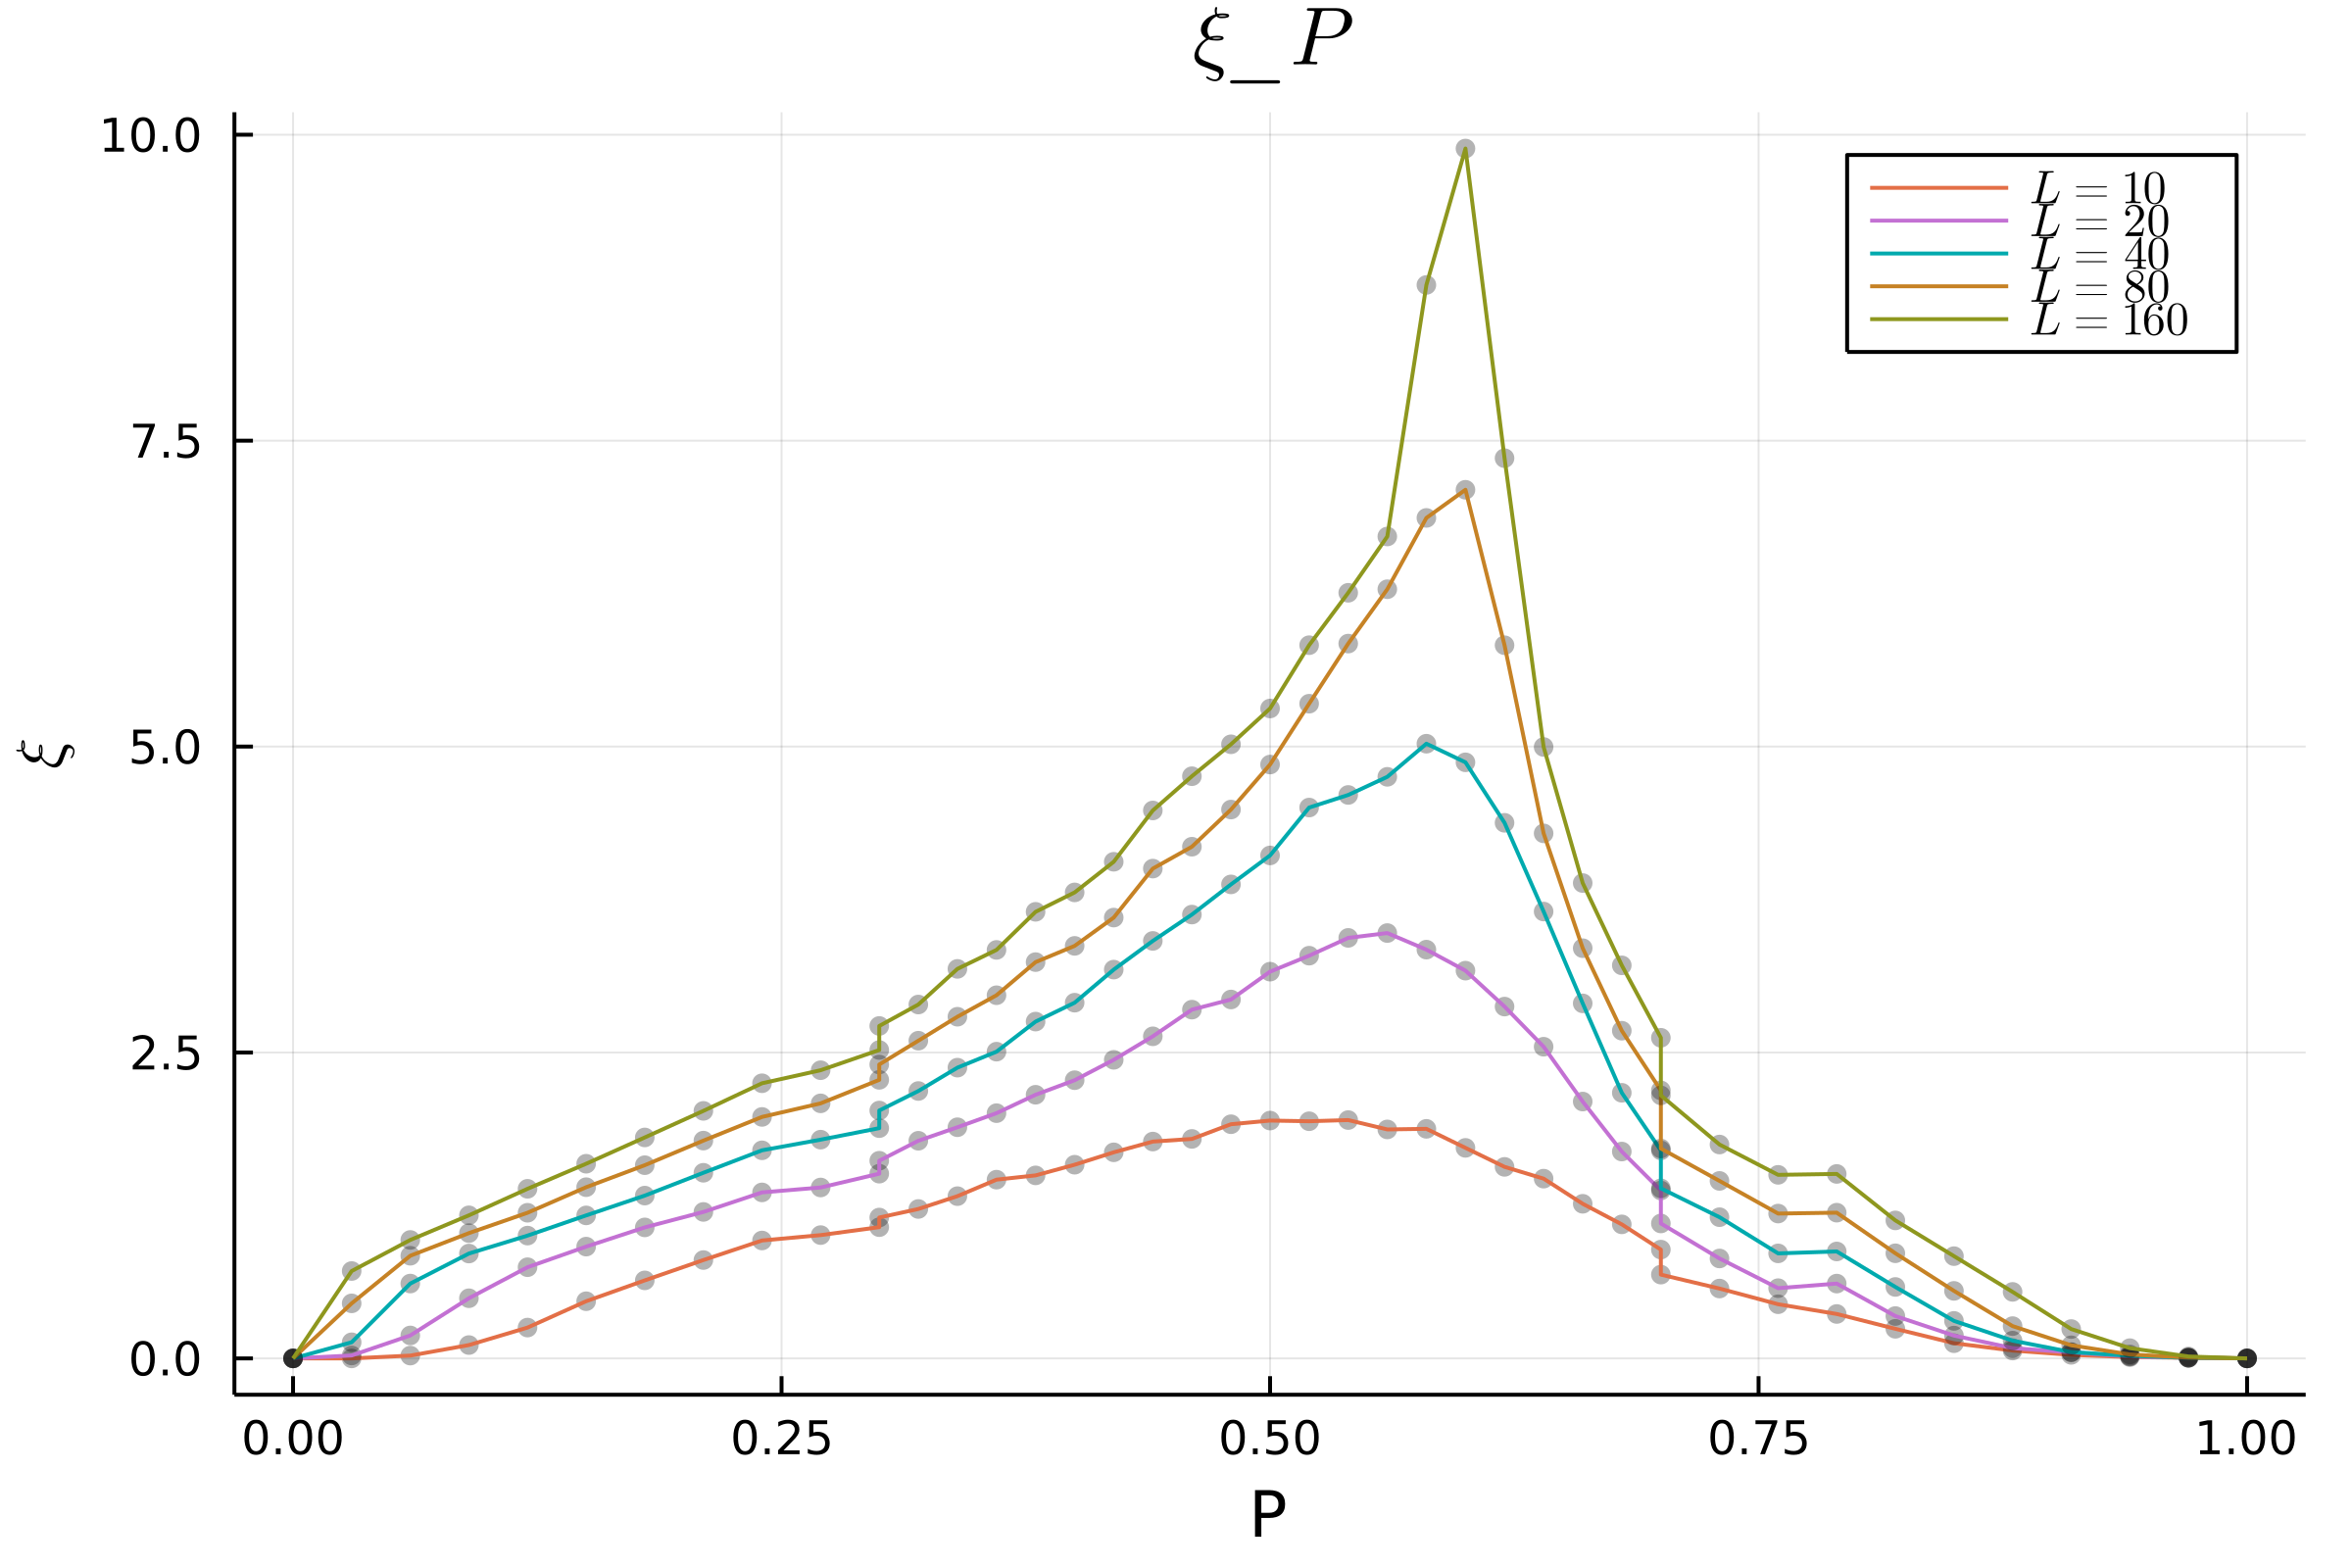
\includegraphics[width=\textwidth]{4.5_plot.png}
		\label{fig:mesh1.2}
		\caption{The plot$\xi$ over probability.}
	\end{subfigure}
	\label{fig:mesh1}
	\caption{The correlation lengths over probability figures of exercise 4.5. probability: $0\leq p \leq 0.25\ (steps=0.03)$,$0.25\leq p \leq 0.75\ (steps=0.02)$, $0.75\leq p \leq 1\ (steps=0.03)$ , Length List= [10,20,40,80,160], Run Number=1000}
\end{figure}

\part*{2. Exercise 4.7: Cluster Growth Algorithm }
\paragraph*{} The overall explanation for this code is that, the program loops through each entry of the matrix, finding that entry which is empty (\textit{zero}) and has at least one \textit{ON} neighbor; After adding this entry to the list of entries that have the same characteristic, each member of the list are sent to the function \textit{on$\_$or$\_$block}, becoming either \textit{ON (represented with 1)} or \textit{Blocked (represented with -1)}, by a given probability. The operation stops when the cluster is blocked either by the boundaries or the blocked entries. 
\paragraph*{} The correlation lengths and the size of the clusters for the given probabilities, averaged over 100 runs are saved in the \textit{"ClusterGrowth$\_$S$\_$xi.jld"} file. 
\begin{figure}[H]
	\centering
	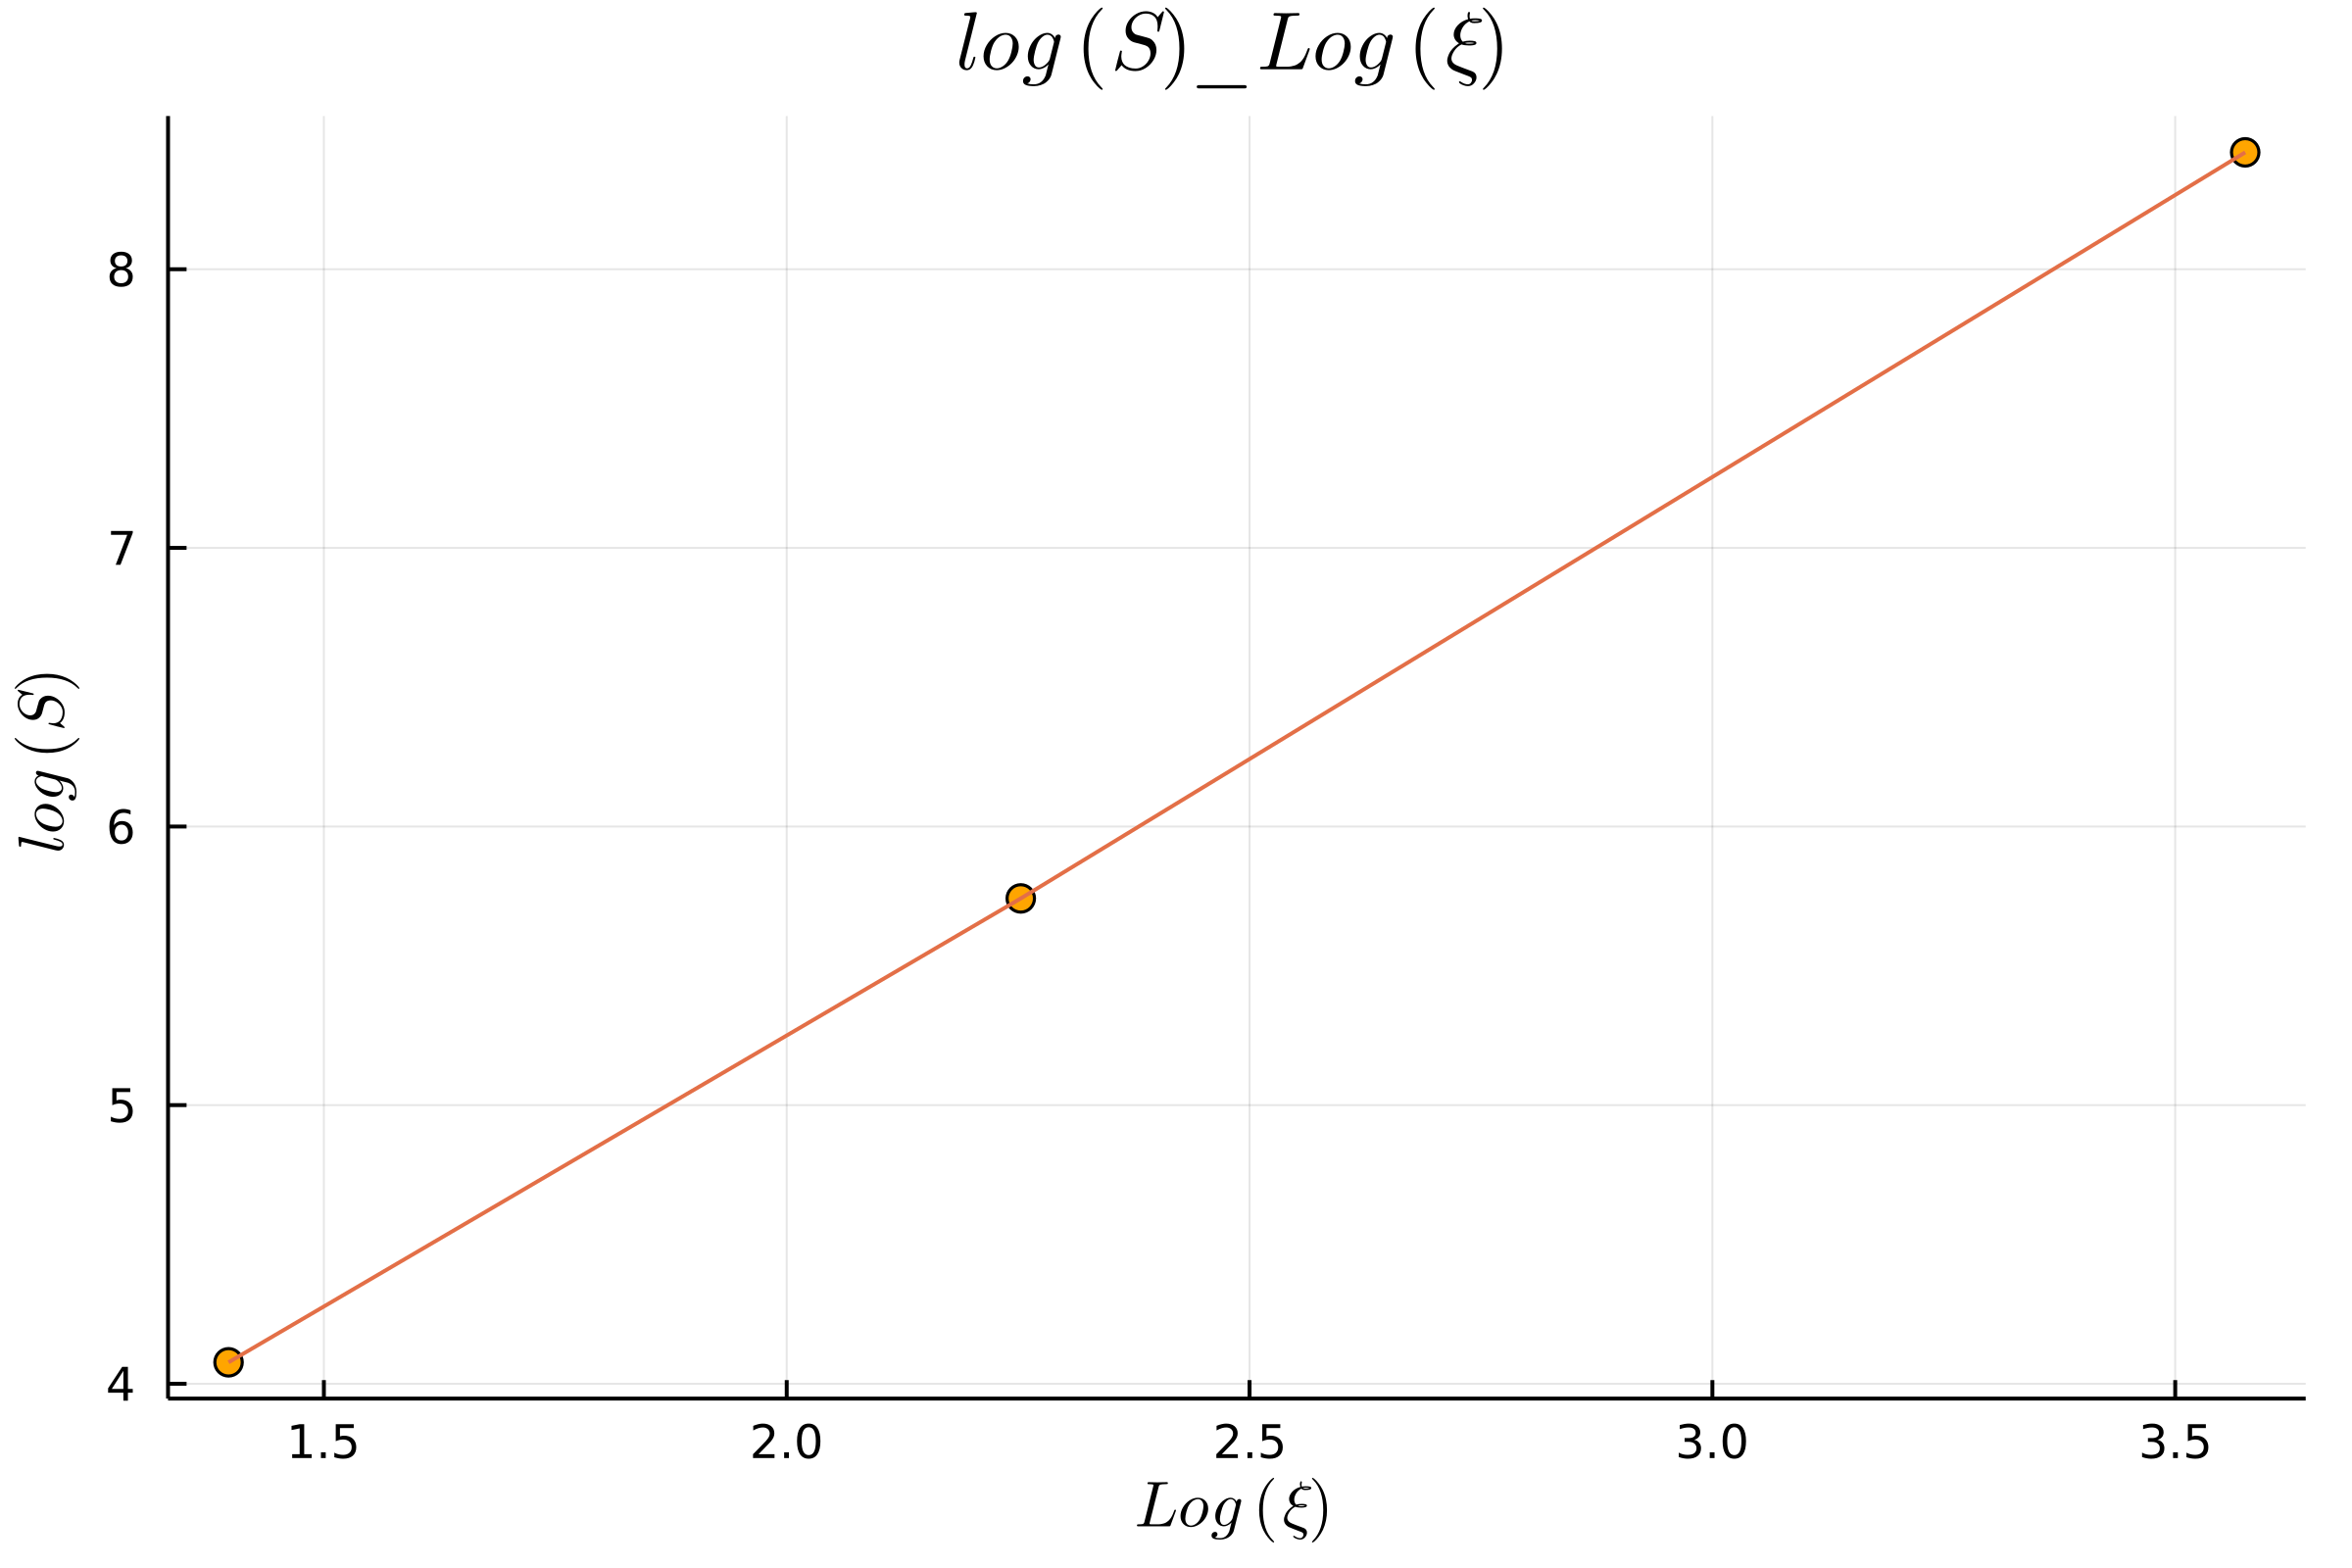
\includegraphics[width=0.7\textwidth]{4.7_log(s)_log(xi).png}
	\label{fig:mesh2}
	\caption{The log(S) over log($\xi$) plot for exercise 4.2.the list of probability=[0.5, 0.55,0.59], Run Number=100.As it's clear from the figure, a line can be plotted passing through the points.}
\end{figure}
\part*{3. Exercise 4.1}
$\left\langle x^{2}(t)\right\rangle=\left\langle(x(t-\tau)+a l)^{2}\right\rangle$
$=\left\langle x^{2}(t-\tau)+2 a l x(t-\tau)+a^{2} l^{2}\right\rangle$\\
$=\left\langle x^{2}(t-\tau)\right\rangle+2 l\langle a\rangle\langle x(t-\tau)\rangle+l^{2}\left\langle a^{2}\right\rangle$ $=\left\langle x^{2}(t-\tau)\right\rangle+2 l(p-q)\langle x(t-\tau)\rangle+l^{2}(p+q)$\\
$=\left\langle x^{2}(t-\tau)\right\rangle+2 l(p-q)\left(\frac{l}{\tau}(p-q)(t-\tau)\right)+l^{2}(p+q)$\\
$=l^{2} \frac{t}{\tau}\left((p-q)^{2}\left(\frac{t}{\tau}+1\right)-2(p-q)^{2}+(p+q)\right)$ 

$\sigma^{2}(t)=\left\langle x^{2}(t)\right\rangle-\langle x(t)\rangle^{2}$\\
$=l^{2} \frac{t}{\tau}\left((p-q)^{2}\left(\frac{t}{\tau}+1\right)-2(p-q)^{2}+(p+q)-(p-q)^{2} \frac{t}{\tau}\right)$\\
$=l^{2} \frac{t}{\tau}\left(p-p^{2}+q-q^{2}+2 p q\right)$ $=l^{2} \frac{t}{\tau}(p q+q p+2 p q)$\\
$=\frac{4 l^{2}}{\tau} p q t$


\part*{4. Exercise 4.2: Random Walk}
\paragraph*{} I consider the dynamics a matrix, which one dimension represents the time steps and the other probabilities. In other words, each column is one walker's changing positions to left and right in a total time of 1000. The entries of the matrix are filled with the given probabilities with 1 ( right) and with -1 (left) at once at the beginning.  At the end using \textit{cumsum}, the matrix of positions at each time, is returned to the a for loop, to repeat for 10000 runs. The position mean and variance per time is listed in a list for arbitrary probabilities, and the figures are plotted. 
\begin{figure}[H]
	\centering
	\begin{subfigure}[t]{0.65\textwidth}
		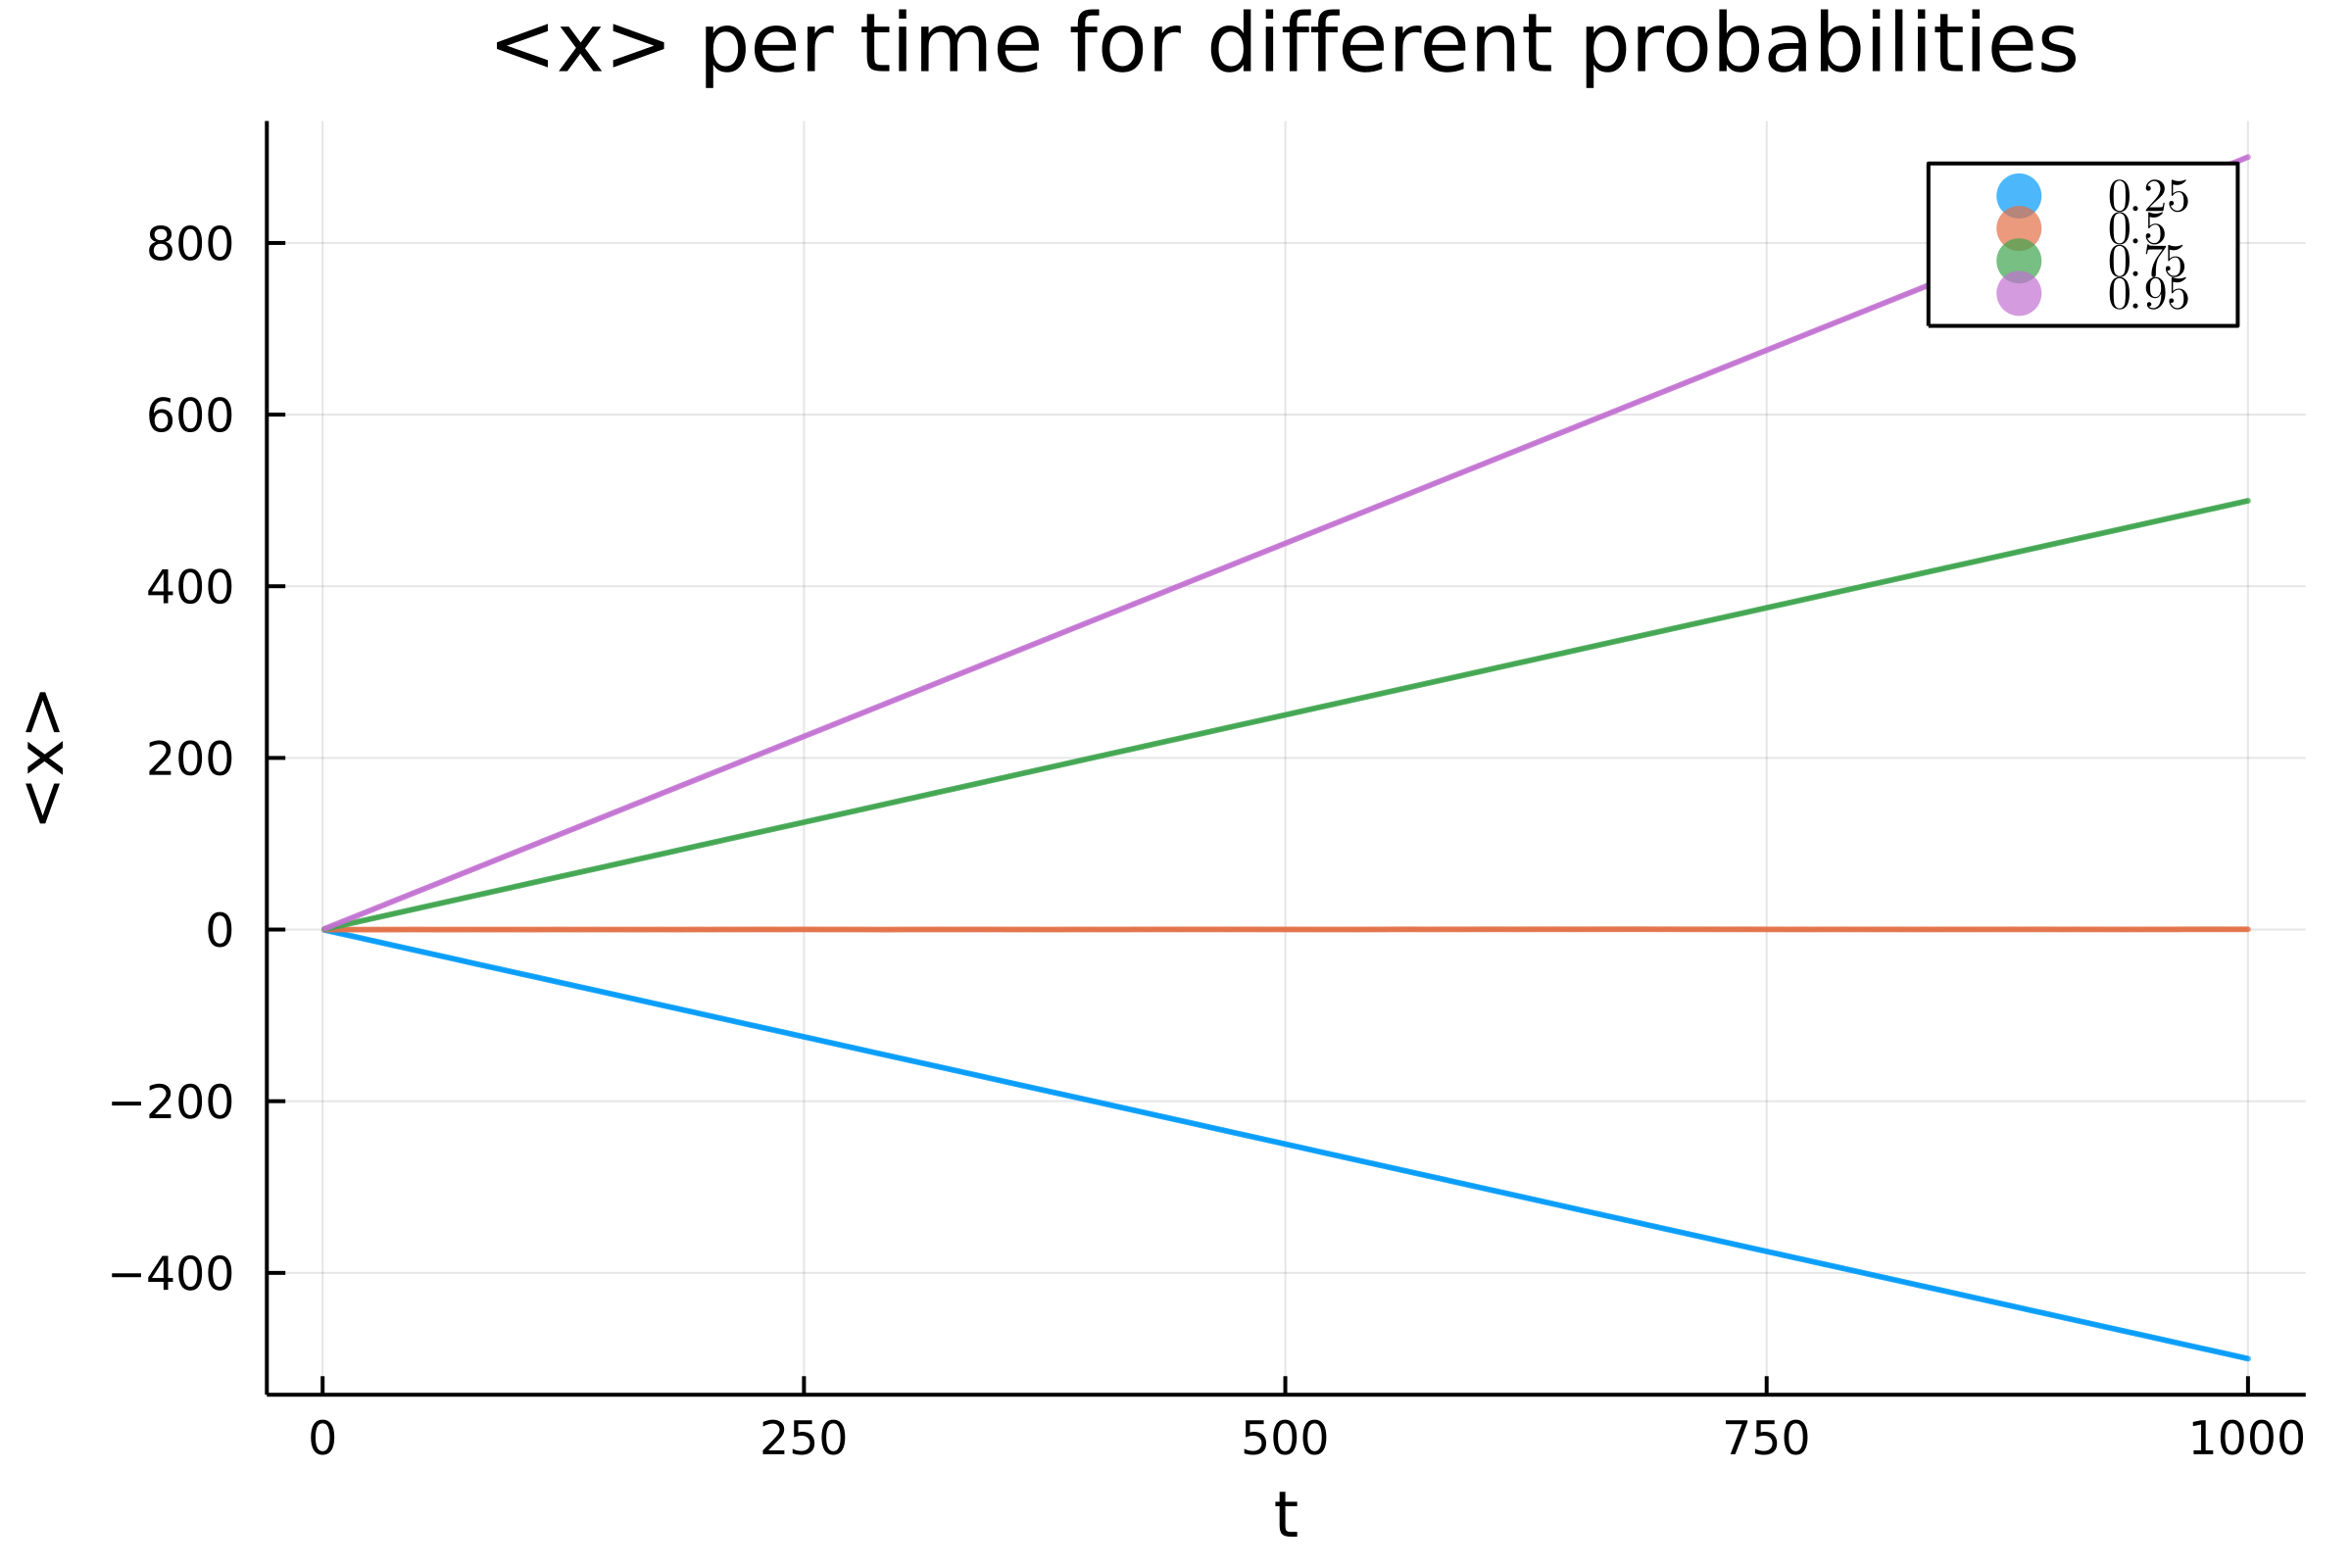
\includegraphics[width=\textwidth]{MeanPlot.png}
		\label{fig:mesh1.1}
		\caption{}
	\end{subfigure}\par\bigskip 
	\begin{subfigure}[t]{0.65\textwidth}
		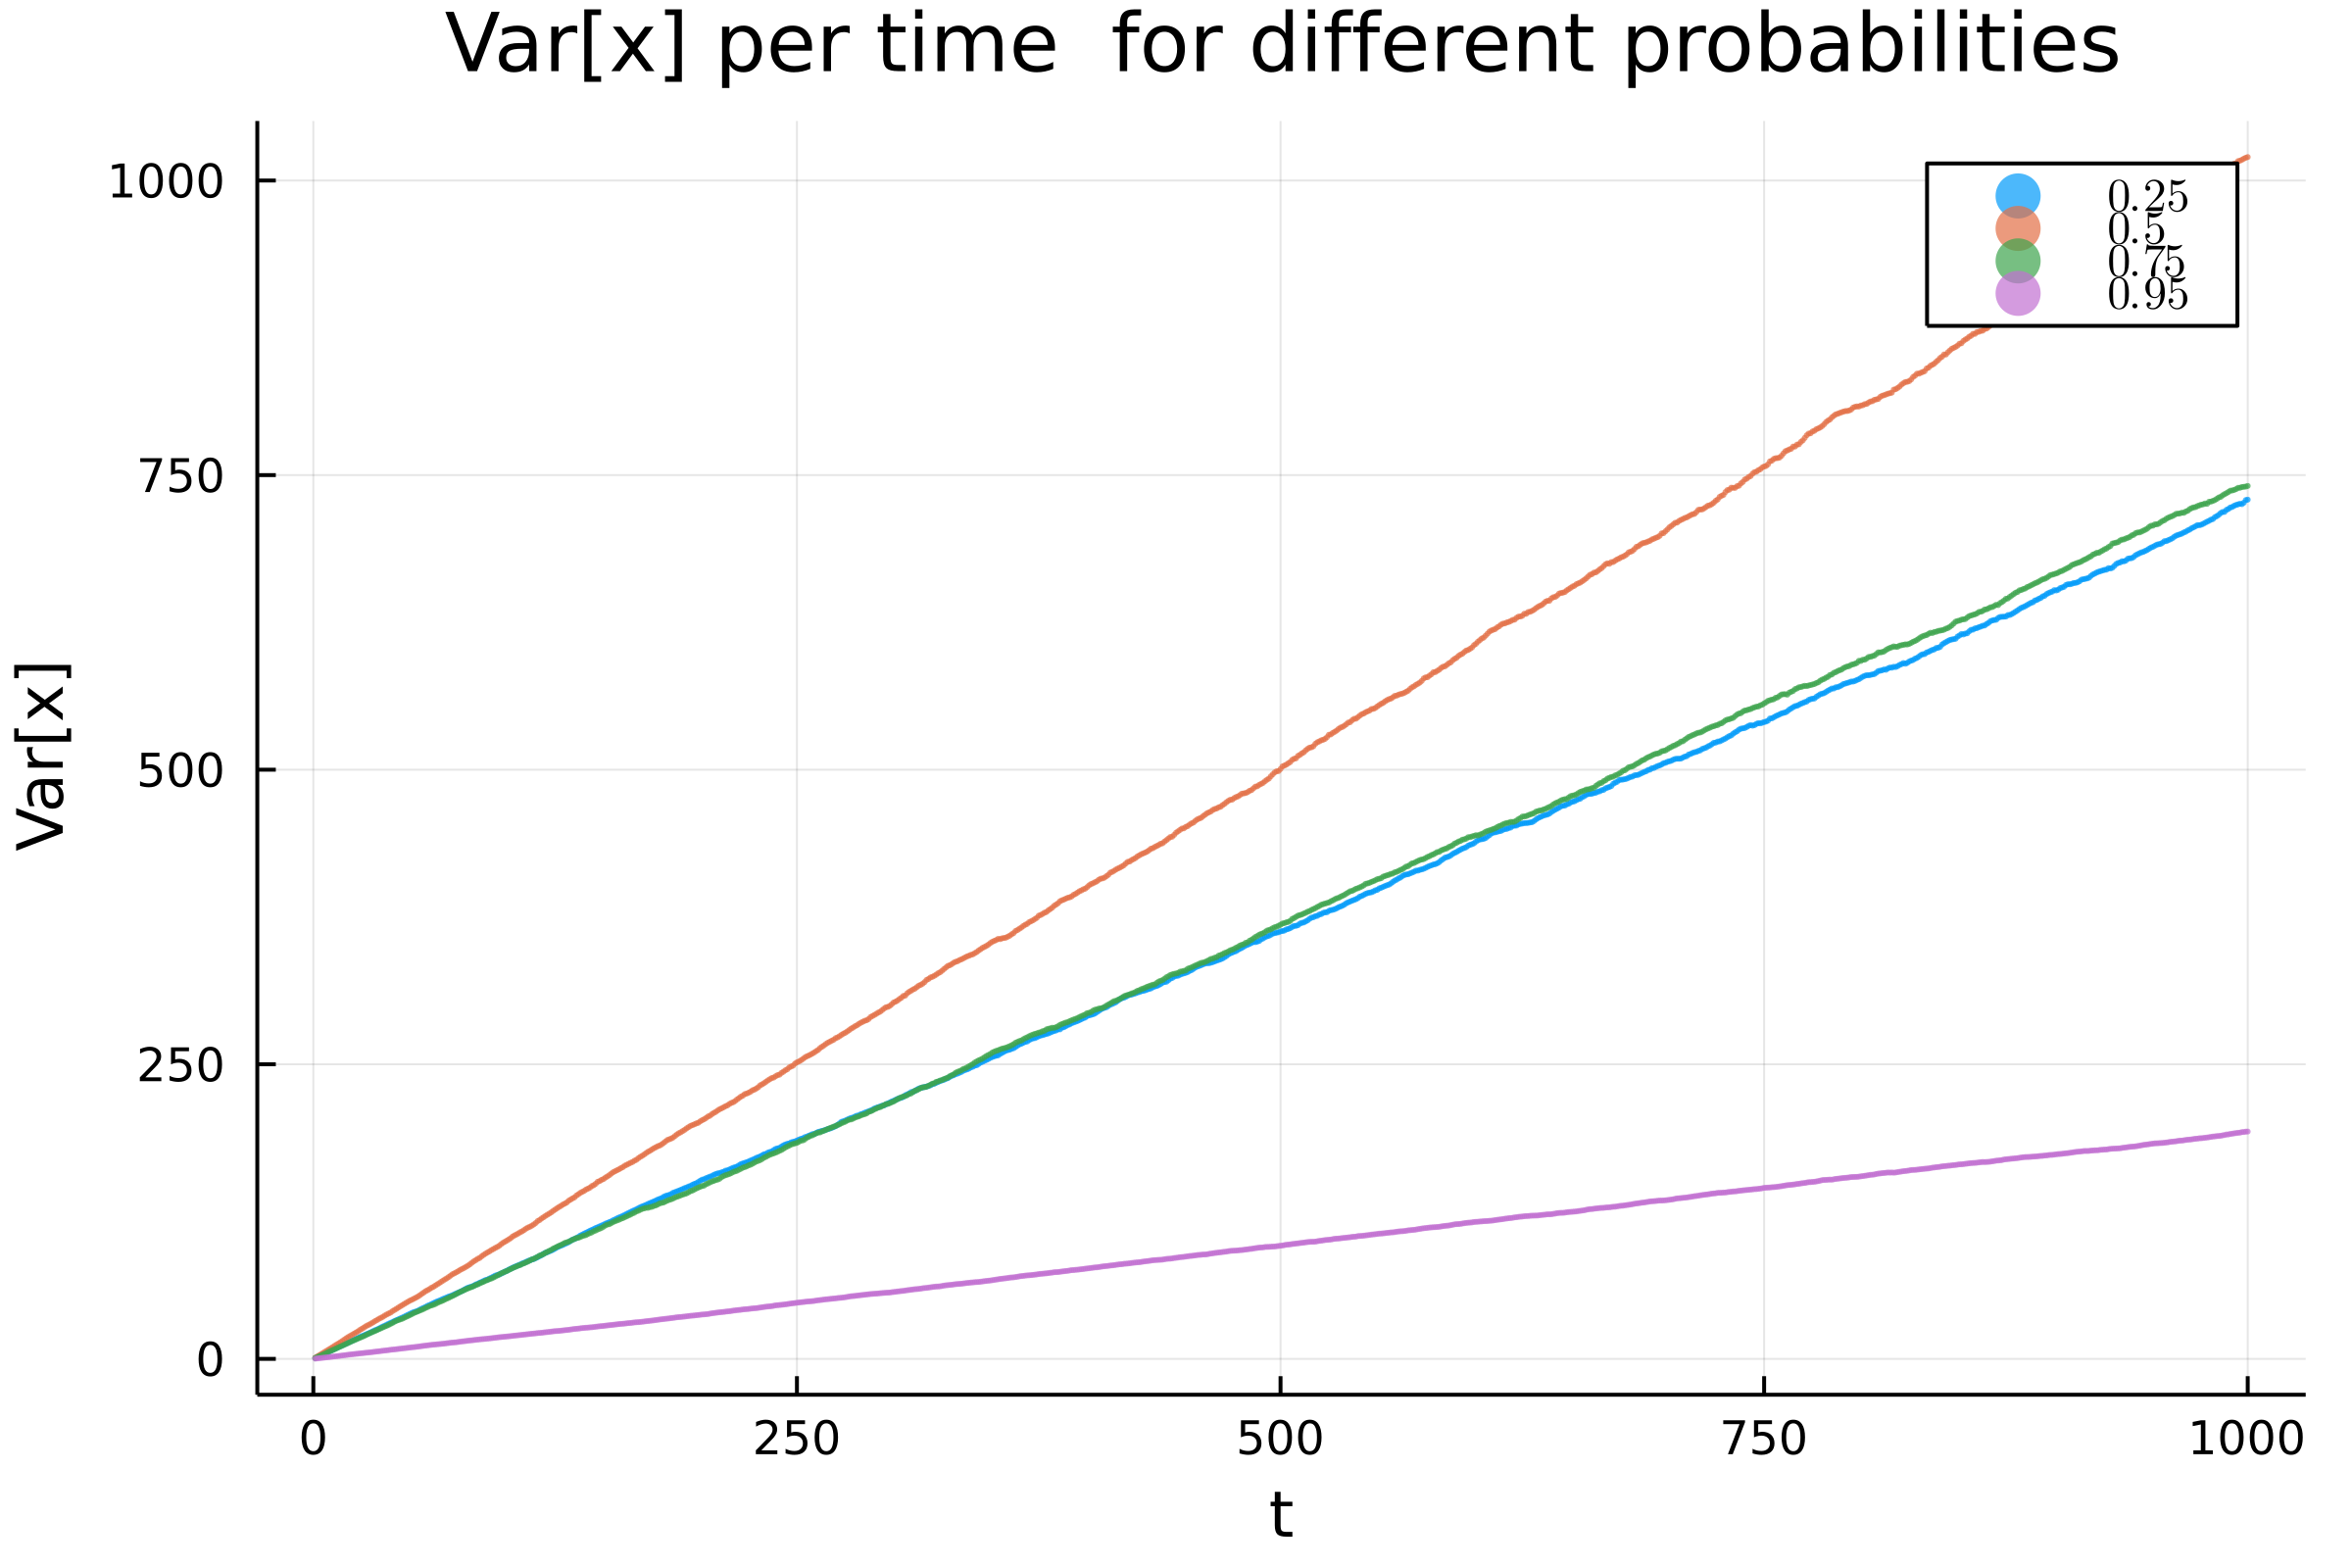
\includegraphics[width=\textwidth]{VarPlot.png}
		\label{fig:mesh1.2}
		\caption{}
	\end{subfigure}
	\label{fig:mesh1}
	\caption{$\langle x \rangle$ and variance(x) over time. Total time=1000, Run Number=1000, list of probabilities =[0.25,0.5,0.75,0.95]}
\end{figure}
\part*{5. Exercise 4.3:Random Walk with Traps}
\paragraph*{} I considered each walker's movements being ordered in a one dimensional array. This time in order to stop the the random walker when reaching the boundaries, we cannot fill the entries at once! It should be done step by step. 
After each step, the cumulative sum is being calculated instantly to check whether we have reached the positions -10 or 10 yet. If not, the loop continues, but if yes, then the resulting array is returned to a loop to repeat the process for 100000 times for each starting position. 
\begin{figure}[H]
	\centering
	\begin{subfigure}[t]{0.8\textwidth}
		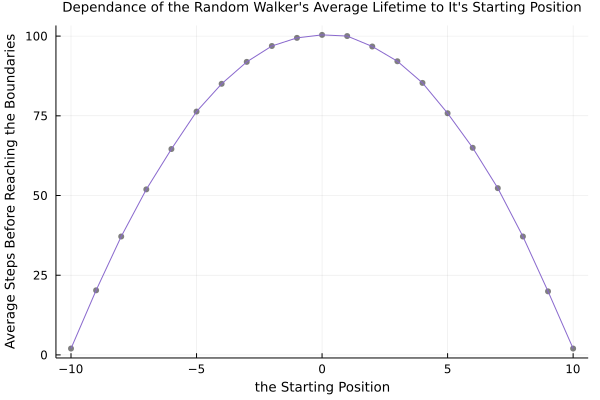
\includegraphics[width=\textwidth]{avgstep_startpos_p=0.5.png}
		\label{fig:mesh1.1}
		\caption{}
	\end{subfigure}
	\begin{subfigure}[t]{0.45\textwidth}
		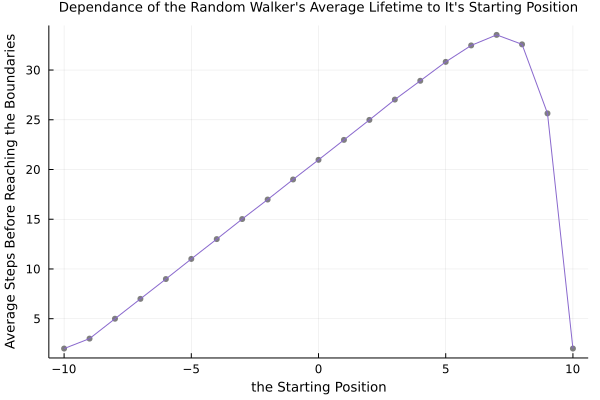
\includegraphics[width=\textwidth]{avgstep_startpos_p=0.25.png}
		\label{fig:mesh1.2}
		\caption{}
	\end{subfigure}\hfill
		\begin{subfigure}[t]{0.45\textwidth}
		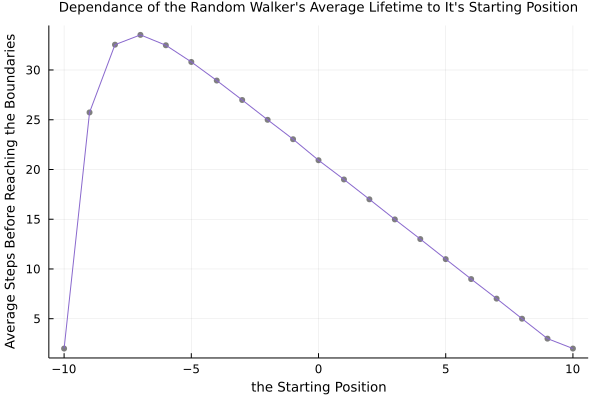
\includegraphics[width=\textwidth]{avgstep_startpos_p=0.75.png}
		\label{fig:mesh1.2}
		\caption{}
	\end{subfigure}
	\label{fig:mesh1}
	\caption{Average steps before falling into the traps over the starting position for (a) p=0.5, (b) p=0.25 and (c) p=0.75 for 100000 walkers. Starting position in range form -10 to 10.}
\end{figure}
\part*{6. Exercise 4.4: Random Walk with Traps(Deterministic Algorithm)}
\paragraph*{} According to this algorithm we should produce the table mentioned in the textbook. So, I created a list, consisting of the probabilities in each step. In every step, a \textit{for loop} goes through each entry of the \textit{R list}, which initially is set to be zero. Every value of the previous step's probabilities is divided by 2 and added with the previous and the next entries' values in this step's list. 
\paragraph*{} The first and the last entries in each step add with the first and the last step's entries, respectively. These entries are the traps.
\paragraph*{} The process goes on until the sum of the traps in each step (the death probability) become a number near to 1, which I assumed to be 0.99999999. 
\paragraph*{} The mean life-span is set to zero initially and adds with the sum of the life-probabilities in every step. 
\begin{figure}[H]
	\centering
	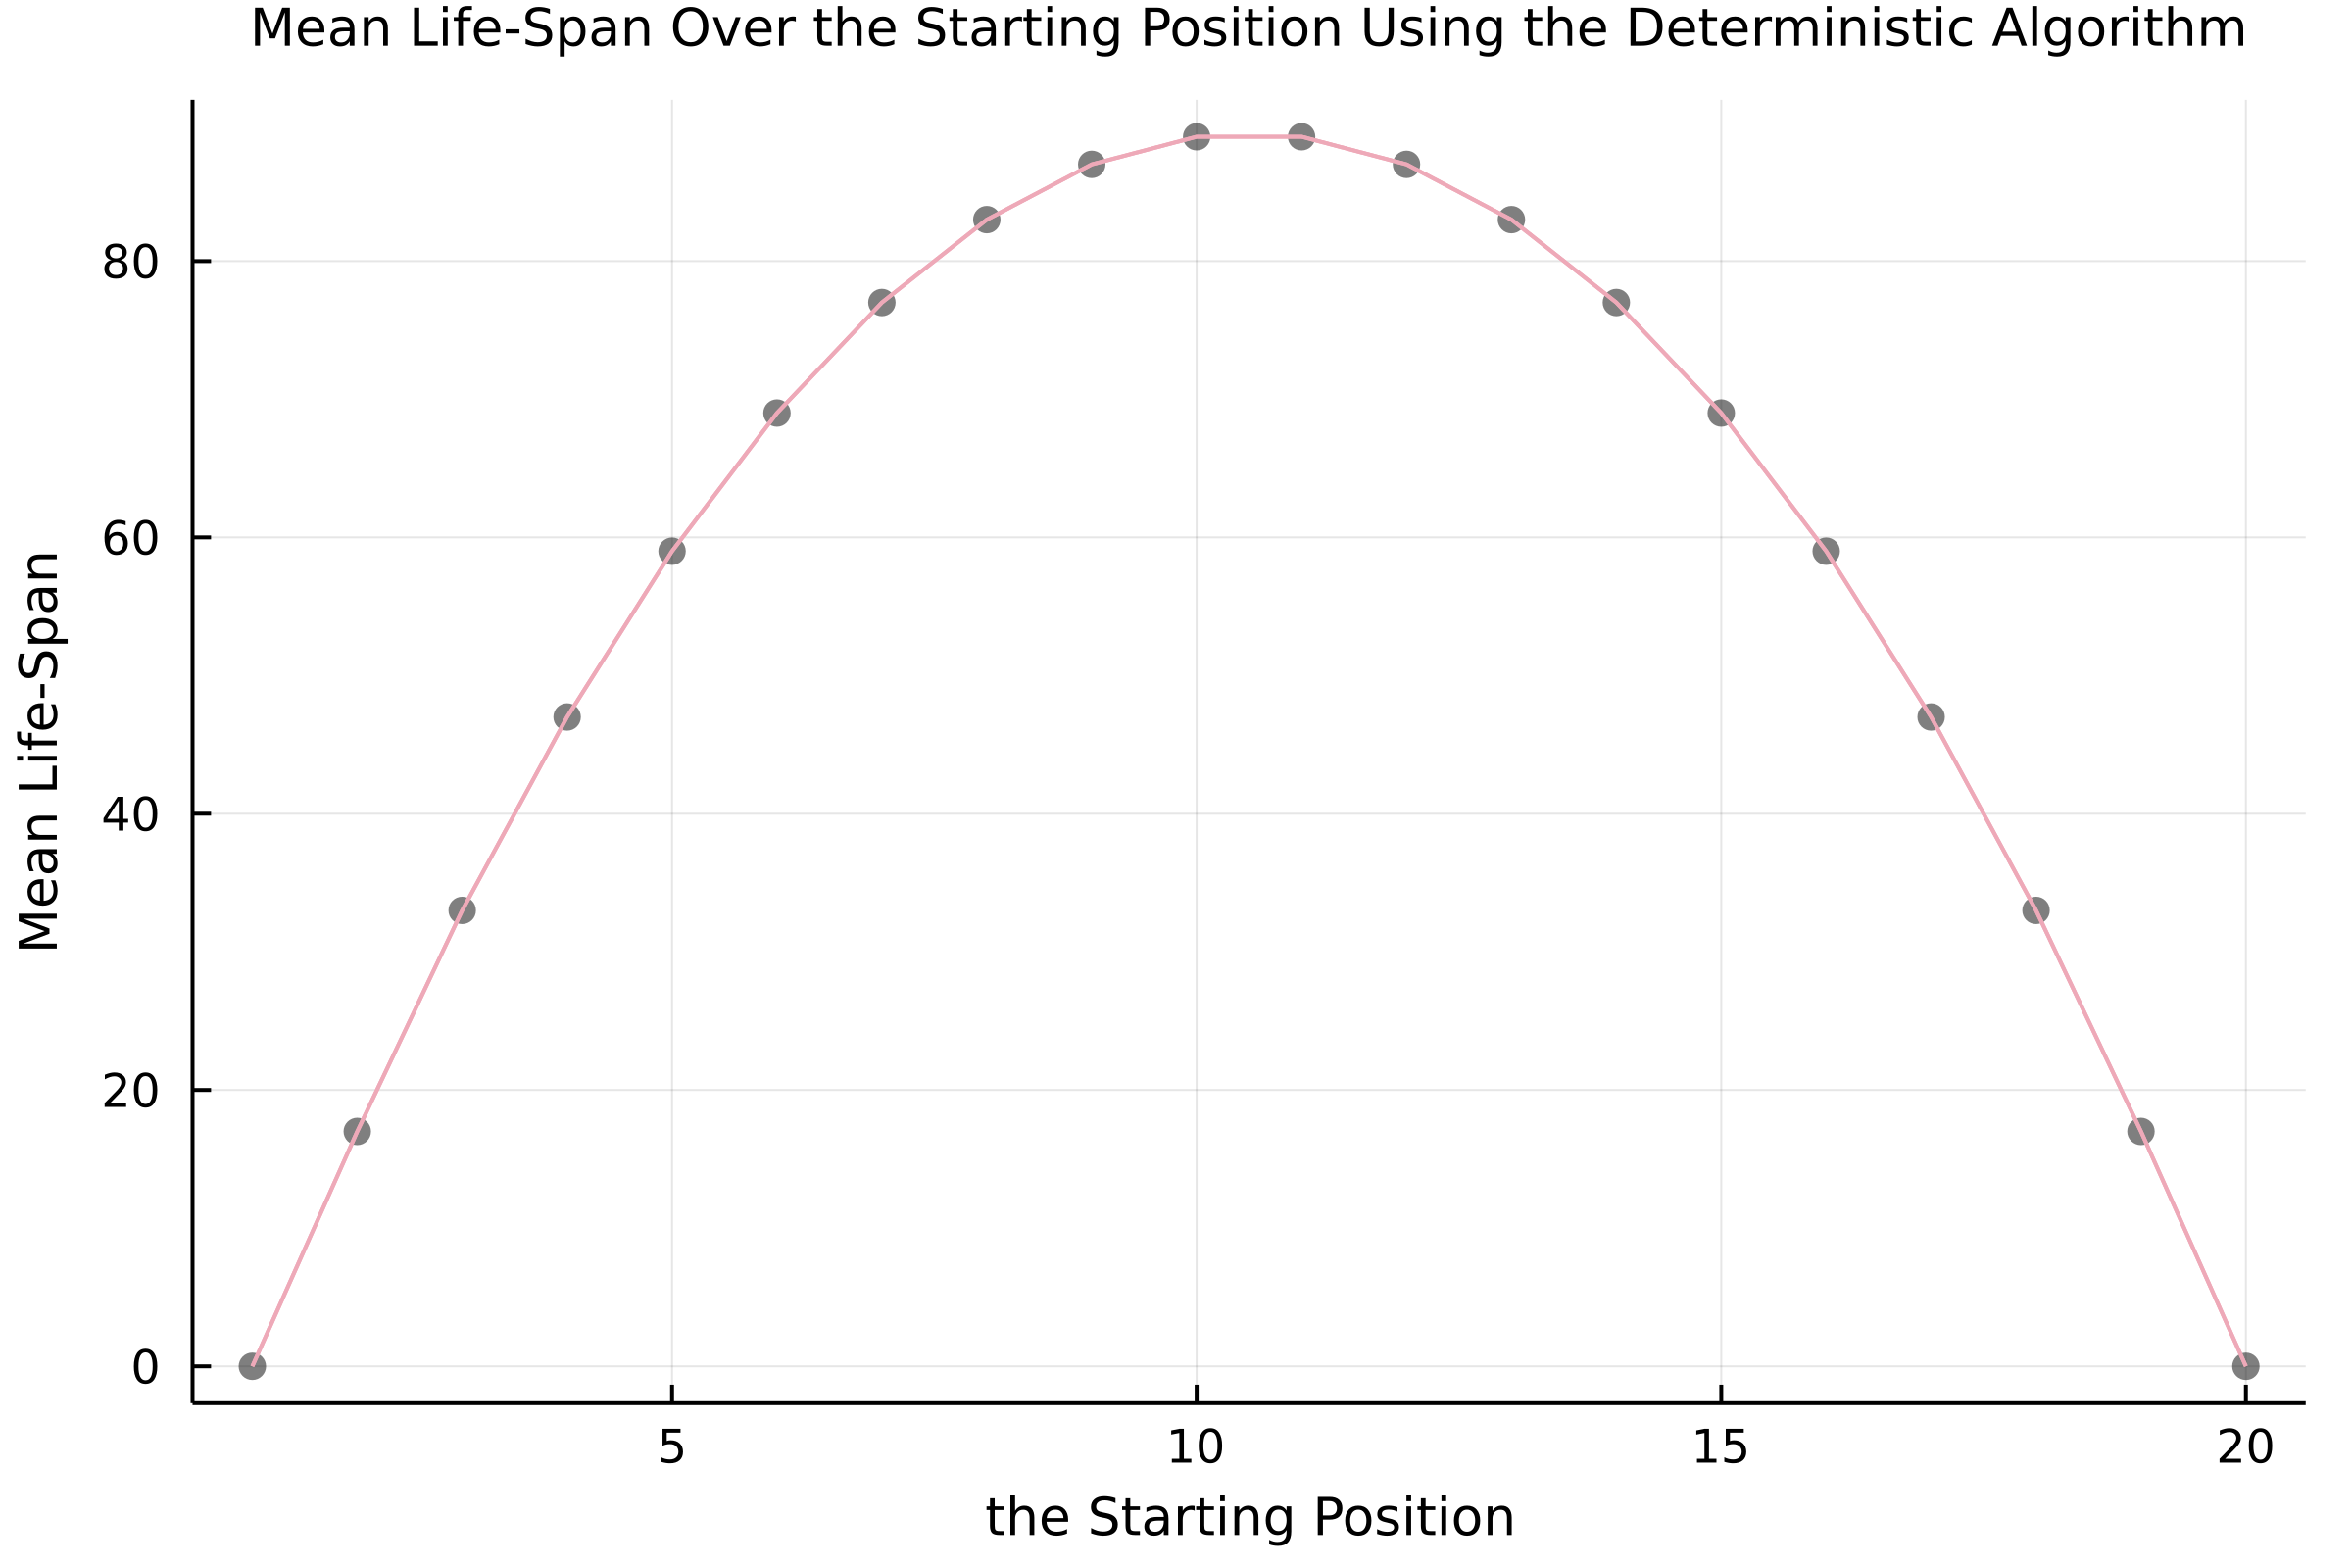
\includegraphics[width=0.7\textwidth]{MeanLifeSpan_startpos_deterministic.png}
	\label{fig:mesh2}
	\caption{The mean life$\_\ $span of each walker over the starting positions ranging from 1 to 20. The run-time is significantly less than the previous algorithm's run-time, and the results are both the same, obviously.}
\end{figure}
\end{document}